I prodotti per la gestione centralizzata dei \textit{log} offerti dal mercato sono svariati, ognuno presenta peculiarit� che lo rendono

ce ne sono tanti, alcuni hanno un taglio troppo specifico, ad es. per un linguaggio solo o per un ambiente solo (es. solo mobile)

di seguito ne riportiamo cinque che sono software generici e si adattano ad esigenze diverse e ci hanno ispirato nella realizzazione di mole.io.

\subsubsection{Airbrake}

\begin{figure}[h]
\centering
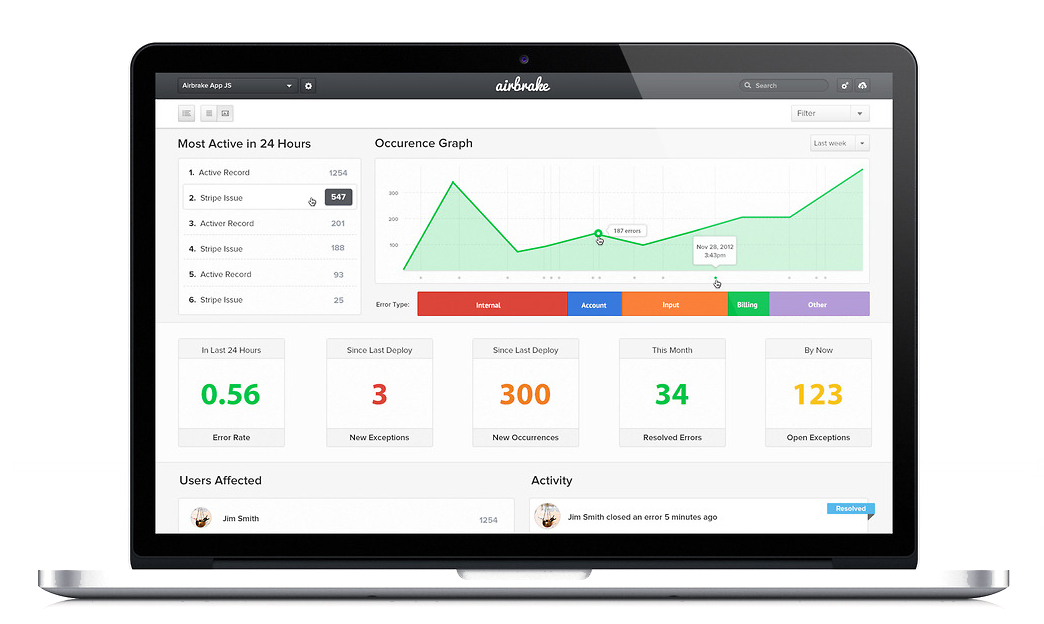
\includegraphics[width=1.0\linewidth]{./img/airbrake}
\caption[Il sito web di Airbrake]{Il sito web di Airbrake}
\label{fig:airbrake}
\end{figure}

Questa � una delle pi� conosciute applicazioni per il monitoraggio dei log prodotti da applicazioni mobile, in realt� Airbrake offre moduli di integrazione per i principali linguaggi di programmazione e pu� essere utilizzata anche in ambito web o desktop.

A partire dalla versione 2.0 propone un pannello di gestione, ricerca e aggregazione dei messaggi di errore completamente rinnovato. L'interfaccia grafica � gradevole e ben organizzata.

Oltre all'aggregazione automatica dei messaggi d'errore, Airbrake possiede moduli di integrazione con i maggiori sistemi di \textit{bug-tracking}, permettendo di attivare \textit{task} per gli sviluppatori alla ricezione di una segnalazione di errore.

Il formato dei messaggi di errore inviabili a questo \textit{tool} � fisso e non permette l'aggiunta di dati addizionali, questo lo rende abbastanza scomodo quando si vogliano tracciare eventi diversi dagli errori.

\subsubsection{Log.io}

\begin{figure}[h]
\centering
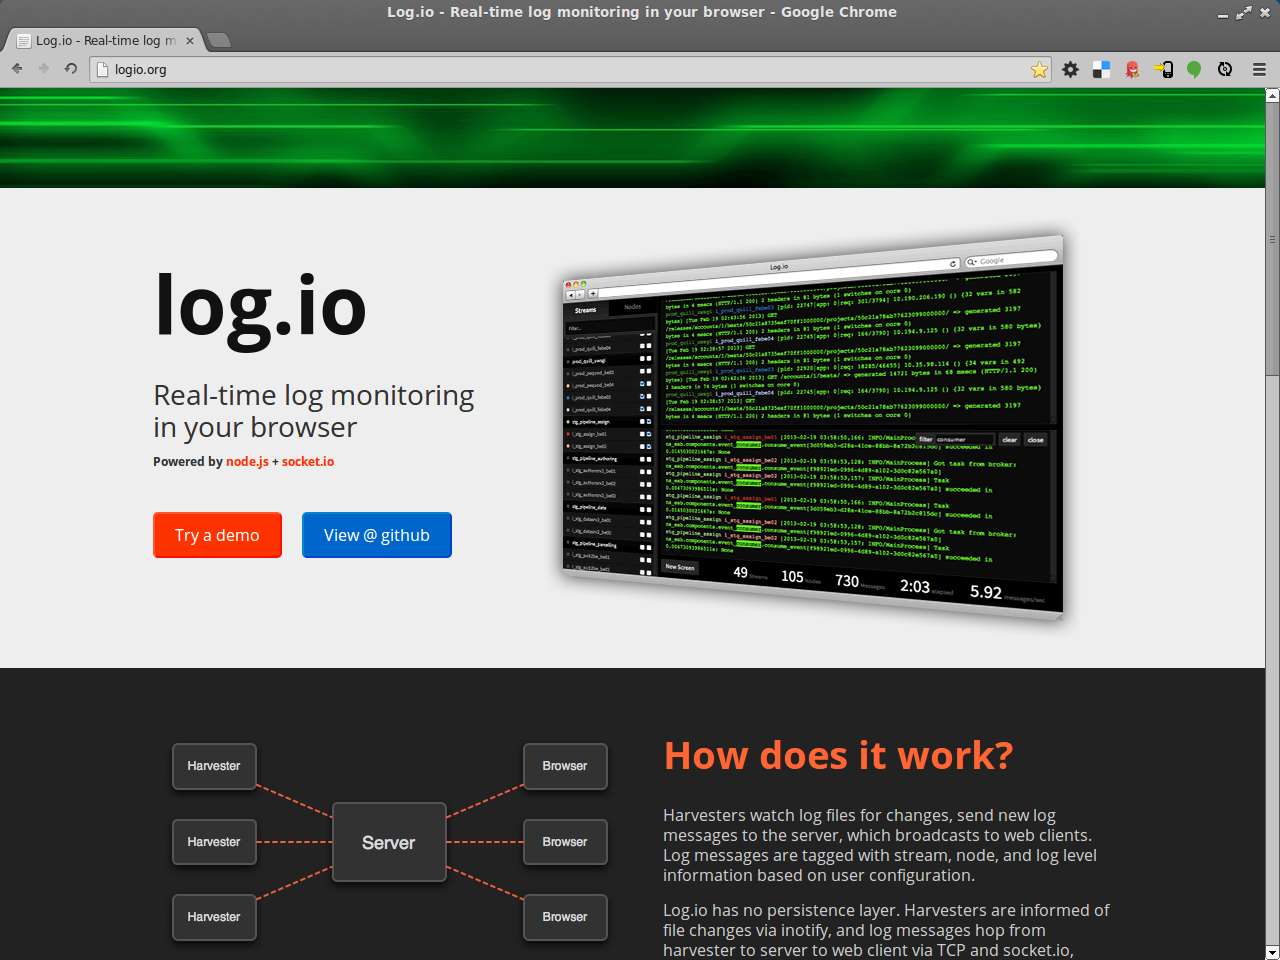
\includegraphics[width=1.0\linewidth]{./img/logio}
\caption[Il sito web di Log.io]{Il sito web di Log.io}
\label{fig:logio}
\end{figure}

La peculiarit� di questo servizio � l'aspetto \textit{realtime}, infatti esso permette di ottenere in tempo reale i log in arrivo dalle applicazioni monitorate.

L'invio dei messaggi al server, da parte delle applicazioni monitorate, avviene tramite messaggi TCP con una formattazione fissa, rendendo questo strumento abbastanza scomodo quando si intende notificare informazioni pi� strutturate di una semplice stringa di testo.

I log vengono gestiti come flussi di dati, � possibile applicare alcuni filtri per limitare la quantit� di informazioni riportate ai soli dati utili all'utente. Purtroppo questo sistema non esegue alcun tipo di aggregazione dei dati in arrivo e non permette quindi di avere una visione d'insieme della situazione dell'applicazione monitorata.

\subsubsection{Rollbar}

\begin{figure}[h]
\centering
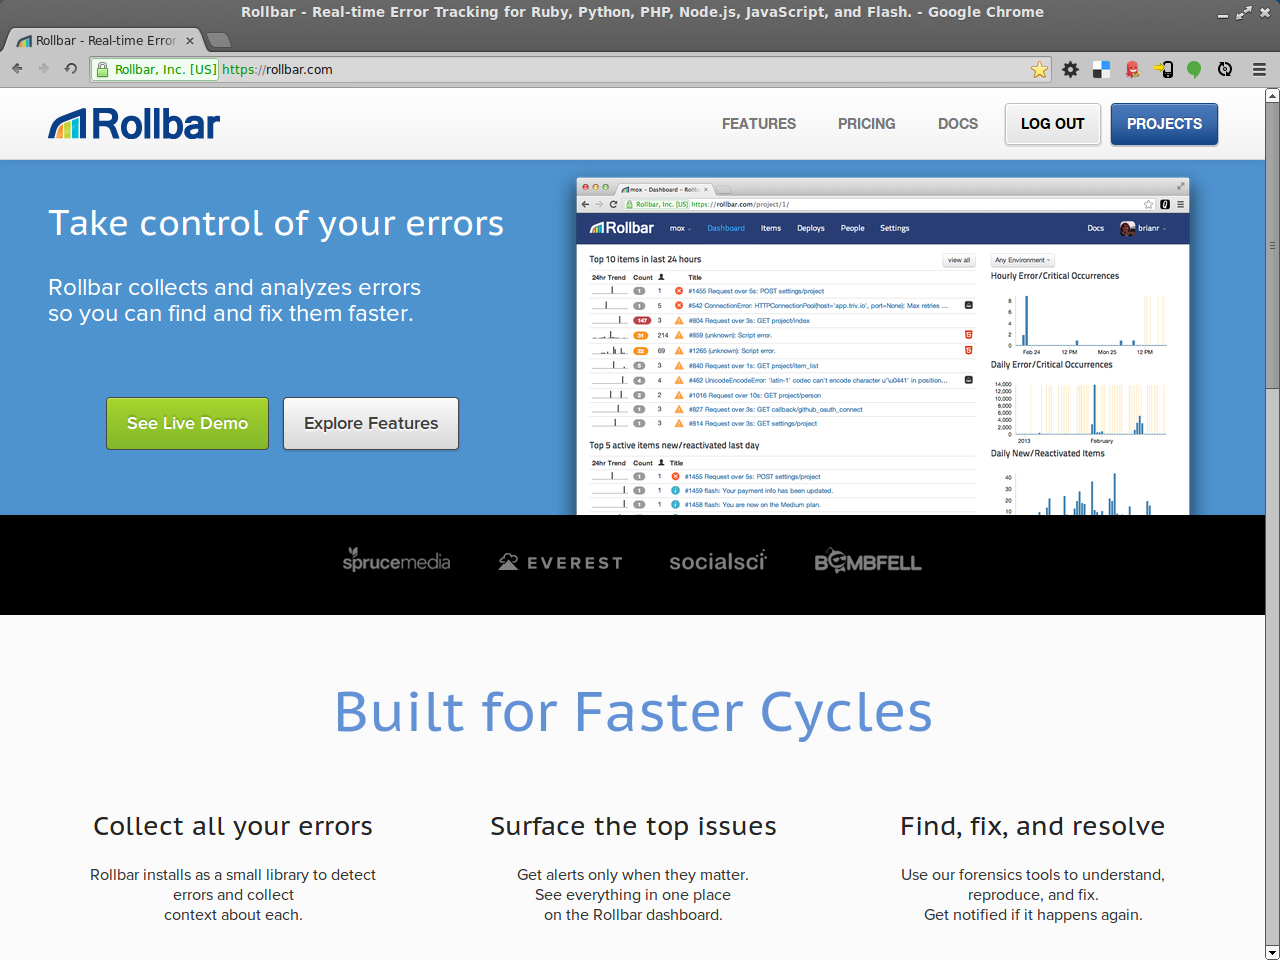
\includegraphics[width=1.0\linewidth]{./img/rollbar}
\caption[Il sito web di Rollbar]{Il sito web di Rollbar}
\label{fig:rollbar}
\end{figure}

Tra le applicazioni a pagamento censite, questa sembra essere la pi� completa, permette infatti di registrare sia messaggi di errore sia messaggi generici.

E' possibile arricchire i messagi inviati a Rollbar con alcuni dati semplici o strutturati definibili dall'utente. L'aggregazione che questo sistema opera su tali messaggi, per�, si limita solo ad alcuni campi obbligatori. 

In questa applicazione � inoltre possibile configurare la notifica via email per alcuni tipi di messaggi e possiede una modalit� di visualizzazione dei dati "realtime".

Permette inoltre di notificare gli eventi aggiungendo automaticamente alcuni \textit{task} nei principali sistemi di \textit{time tracking} e \textit{project management} esistenti sul mercato. 

%da dire: un messaggio ha dati di base (tipo la severity) e dati addizionali tipo messaggi o altri dati strutturati allegabili (stessa idea di mole) ma la gestione non � proprio pulita, 

\subsubsection{Papertrail}

\begin{figure}[h]
\centering
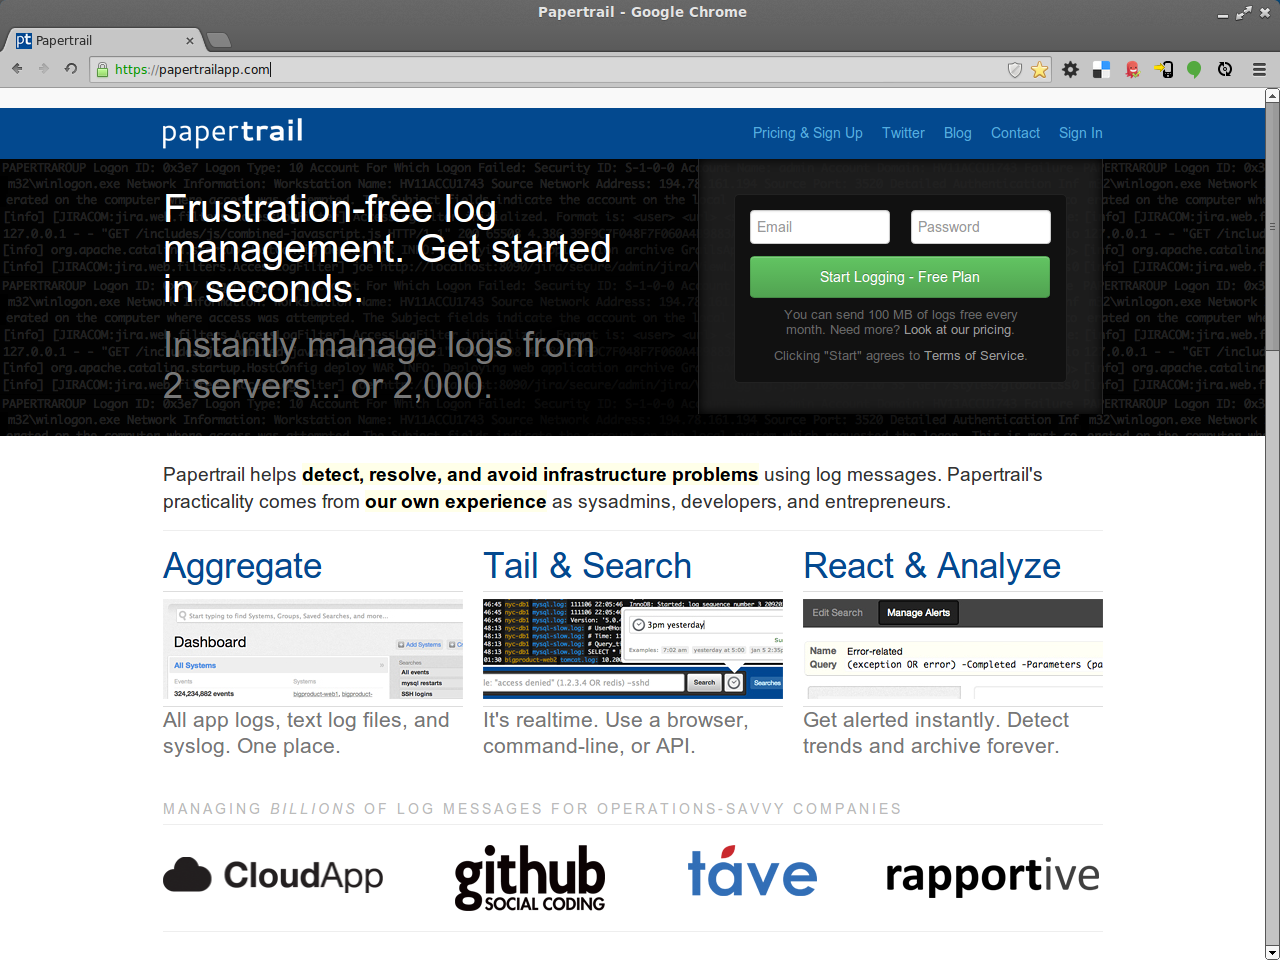
\includegraphics[width=1.0\linewidth]{./img/papertrail}
\caption[Il sito web di Papertrail]{Il sito web di Papertrail}
\label{fig:papertrail}
\end{figure}

E' un tool molto orientato agli amministratori di rete, permette infatti (lo dice il nome stesso) di eseguire una sorta di \verb|tail| dei messaggi che riceve, permettendo cos� di ottenere la coda degli ultimi messaggi arrivati in tempo reale.

Esegue una aggregazione automatica dei log estrapolando la chiave di aggregazione dal formato stesso del messaggio, ad esempio il server che hai inviato il messaggio, il tipo di traccia (riavvio del sistema, login utente, errore di Apache). 

Gli errori sono ricercabili anche utilizzando delle ricerche temporali.

permette di inviare solo log con formati precisi, non � possibile aggiungere dati utente strutturati.
 
\subsubsection{Fluentd, ElasticSearch e Kibana}

\begin{figure}[h]
\centering
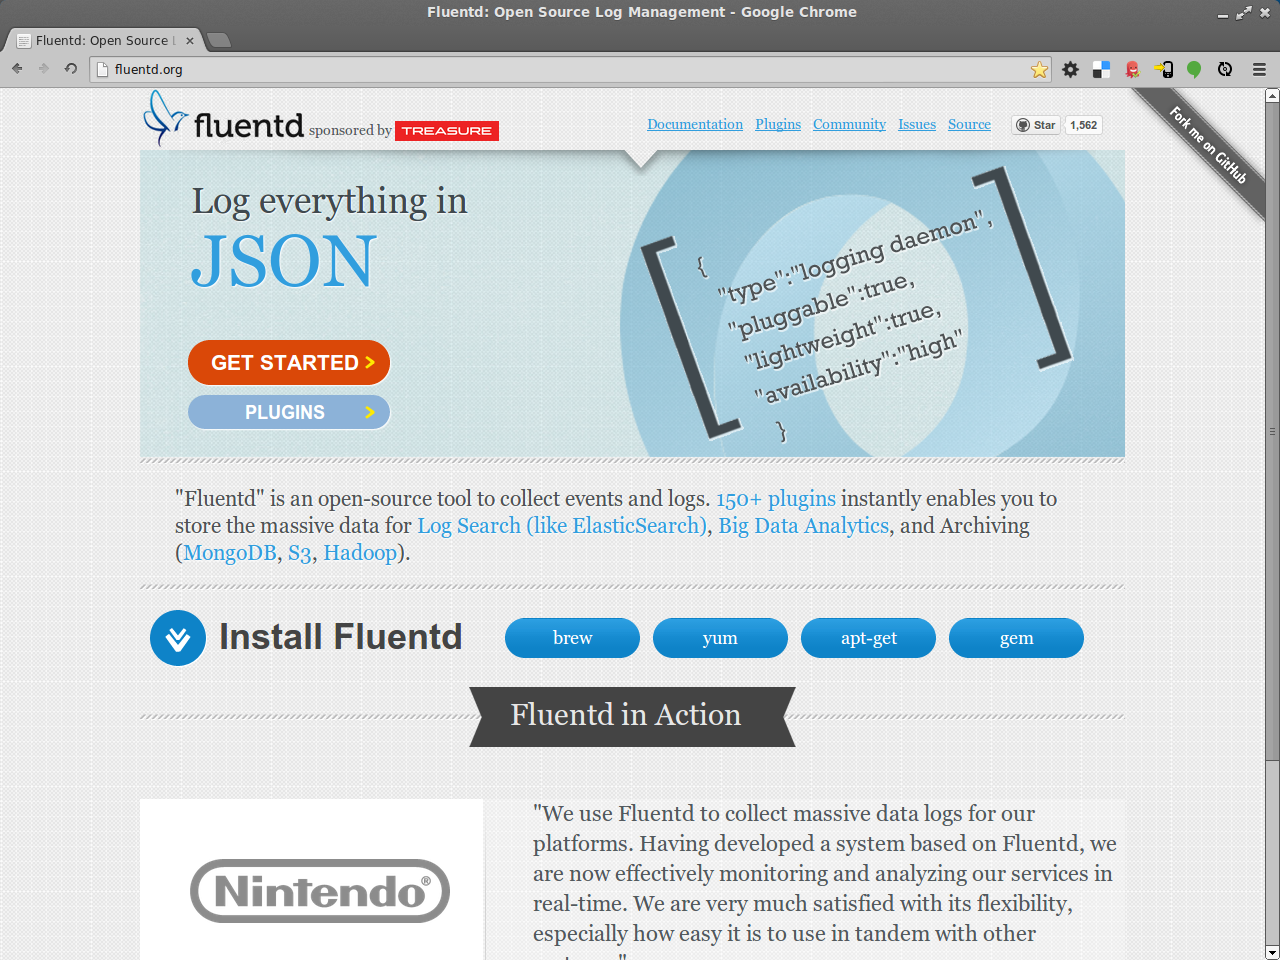
\includegraphics[width=1.0\linewidth]{./img/fluentd}
\caption[Il sito web di Fluentd]{Il sito web di Fluentd}
\label{fig:fluentd}
\end{figure}

\begin{figure}[h]
\centering
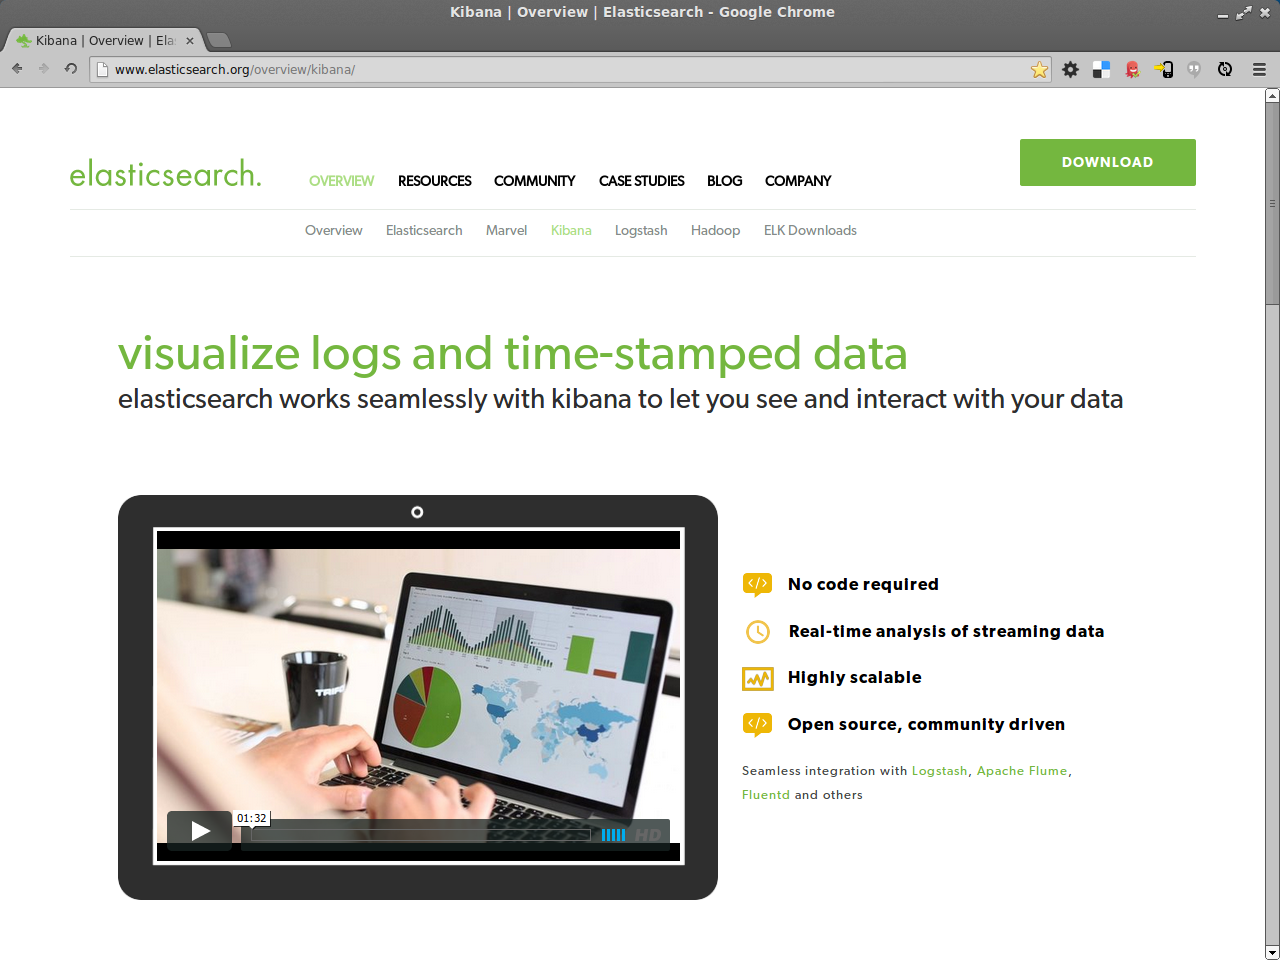
\includegraphics[width=1.0\linewidth]{./img/kibana}
\caption[Il sito web di Kibana]{Il sito web di Kibana}
\label{fig:kibana}
\end{figure}

[soluzione relativamente nuova (?), l'abbiamo trovata durante lo sviluppo.]

Questi sono tre applicativi separati e sono i migliori tra gli open source che abbiamo esaminato.

Per ottenere un logger tipo gli altri vanno utilizzati insieme

Permettono di aggregare dati da sorgenti differenti, anche non messaggi di errore.

la struttura � fluentd > elastic search > kibana

Fluentd � un sistema di raccolta messaggi in formato JSON che supporta infiniti formati, grazie all'utilizzo di plugin.

uno di questi plugin permette di esportare i messaggi ricevuti verso Elastic search: un software che permette di aggregare dati non strutturati. il servre Elastic Search viene infine interrogato dall'interfaccia grafica Kibana che permette di utilizzare widget per mostrare i dati aggregati.

� una soluzione che ti devi "fare in casa" i sw vanno installati e configurati
Esiste un servizio che include gi� tutti gli strumenti, ma � a pagamento.
















overview di alcuni sistemi di logging con le relative funzioni specifiche
i competitor
airbreak - logga solo
rollbar - aggrega
papertrail - live log

sul mercato esistono svariati sistemi per la gestione centralizzata dei log


Airbrake
+
aggrega log e ne facilita l'analisi
integrato con sistemi di tracking 
-
formati dei messaggi fisso e solo errori


log.io
+
realtime
-
no aggregazione

rollbar
+
non logga solo errori, ma la gestione delle "non eccezioni" � un po' tirata per i capelli
fa aggregazione

https://rollbar.com/vs/airbrake/ questo � mooooolto meglio di mole :(

-
soluzione completa ma blindata e non estensibile (gniiiiiii)



papertrail
+
realtime
aggregazione
-
logga solo tipi di errori noti, no formato flessibile







CACCHIO! fluentd + elasticsearch + kibana = mole
%(mole � pi� facile....gniiiiii)



%mole � pensato pi� come una piattaforma espandibile, accento sulla possibilit� di aggiungere features a caldo